\documentclass[a4paper,11pt]{article}

\usepackage{exptech,hyperref}
\hypersetup{
	colorlinks=true,                         
	citecolor=black, % Couleur des numéros de la biblio dans le corps
	urlcolor=blue,   % Couleur des url
	linkcolor=black}  % Couleur des liens internes

%Décommanter pour la relecture (interlignes plus importantes)
%\linespread{1,6}

%%%%%%%%%%%%%%%%%%%%%%%%%%%%%%%%%%%%%%%%%%%%%%%%%%%%%%%%%%%%%%%%%%%%%%%%%%%%%%%

\title{ \textbf{Création d'un modèle 3D à partir de dessins 2D Documentation Technique} }
% Pour avoir le titre de l'expose sur chaque page

\author{ Aurélien \textsc{FONTAINE} Etienne \textsc{GEANTET} \\
	Manutea \textsc{HUANG} Arnaud \textsc{MARTIN} \\
	\\
	Encadrants : François \textsc{LEHERICEY}	Bertrand \textsc{COUASNON}}

\date{4 Mai 2015}                    % Ne pas modifier

%%%%%%%%%%%%%%%%%%%%%%%%%%%%%%%%%%%%%%%%%%%%%%%%%%%%%%%%%%%%%%%%%%%%%%%%%%%%%%%

\begin{document}

\maketitle                 % Génère le titre
\thispagestyle{empty}      % Supprime le numéro de page sur la 1re page

\begin{abstract}
	Notre projet fonctionne sous Unity 4.6.1 en mode éditeur, dû à des parties qui seront détaillées dans la partie du code de l'extrusion.
\end{abstract}

\section{arborescence}
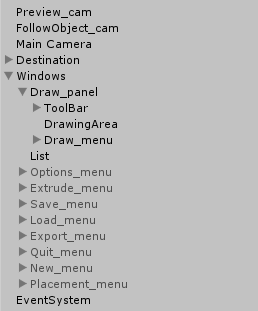
\includegraphics[scale=0.7]{./images/arborescence.png}
		\begin{itemize}
			\item Les trois premiers objets sont les caméras
				\begin{itemize}
					\item Preview\_cam est la caméra qui affiche en permanence en haut à droite le rendu de notre figure
					\item Follow\_ object est la caméra qui suis notre objets quand on le place dans l'environnement 3D
					\item Main camera est la caméra principale
				\end{itemize}
			\item Destination, c'est le contenant de tout les objets que l'ont va crée, c'est lui qui sera transmis par la suite au serveur. Il possède un sous item invisible, car cela posais des problèmes pour la disposition des caméras quand il n'y avais rien. Nous n'avons pas trouver d'où cela venais
			\item Windows, le canvas principal, c'est lui qui est filmé par la Main Camera
			\item Toolbar, barre de menu grise en haut
			\item DrawingArea, zone où l'on dessine
			\item Draw\_menu, menu des outils, il est associé à une animation pour la rentrée/sortie
			\item List, canvas vide qui représente la zone en bas à droite
			\item XXX\_menu, toutes les fenêtres
			\item Placement\_menu, ne suis pas le même modèle que les menus précédant, c'est ce qui permet le placement de la figure dans l'environnement 3D
		\end{itemize}
\section{Dessin}
	\subsection{Draw\_menu}	
		Ce menu est associé à un script	qui permet la gestion des outils. Pour ajouté un outils, il faut crée une fonction sur le même modèle que les setX(), et appeler selectionne() avec le nom du bouton et le type d'outils. 
	\subsection{DrawingArea}
		Ce composant possède un script qui le redimensionne pour l'adapter à l'écran.
		Il possède un script qui gère le dessin, dans ce script on retrouve aussi les fonctions pour rendre actif ou non cette zone: SetIsSelect(int i) et InitIsSelect(), quand isSelected == 0, le dessin est autorisé. La latence permet de ne pas dessiné dessus quand on ferme une fenêtre qui étais devant. C'est cette partie qu'il faut revoir avec le tactile.
		
\section{Previem\_cam}
		Possède un script qui gère le glissement de la souris pour ensuite déplacé la caméra selon cela. Nécessite des corrections pour le tactile.
\section{Placement}
		\subsection{Les objet}
			L'objet Taille fils de Placement\_menu correspond à un coefficient à appliquer aux 3 dimensions de l'objet. Il y a ensuite 3 menu, un pour chaque axe. Chaque menu possède une objet Taille qui lui correspond dà la taille selon un axe orthogonal.
			
			Quand on extrude un objet, tout les menus autre que Placement\_menu sont désactivé et réactivé à la fin. Cela peut crée un léger bug au niveau des animation du Draw\_menu au prochain click dessus.
		\subsection{Les scripts}
			Le placement d'un objet est initialisé dans UclaExtrusion.cs (les lignes concerné on un commentaire adapté). Cette initialisation, comprend l'activation des menu, et le chargement dans la caméra FollowObject\_cam de l'objet à suivre et de passé tout les autres objets en transparence.
			Quand on fait cet initialisation, celle ci initialise le script Translate.cs placé sur l'objet Destination. Ce script permet de déplacer l'objet que l'ont viens de crée avec UclaExtrusion via les boutons de Placement\_menu.
\section{Réseau}
	\subsection{Serveur}
		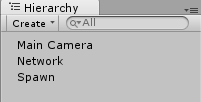
\includegraphics[scale=0.9]{./images/arbserver.png}
		\begin{itemize}
			\item Network contient le script qui gère la création et le comportement du serveur.
			\item Spawn est le point de repère pour faire apparaître l'objet reçu.
		\end{itemize}
		
		Le serveur se lance automatiquement au démarrage de l'application si Spawn et Network ne sont pas masqués.
		\subsubsection{Network et TcpServer}
			Le GameObject Network ne contient que le script "TcpServer".
			
			Le script "TcpServer" est composé essentiellement de 5 fonctions:
			\begin{itemize}
				\item Start : Crée un TcpListener et lance l'attente d'un client dans un thread qui tournera en arrière-plan.
				
				\item ListenForClients : Lance le TcpListener et attend qu'un client se connecte. Dès qu'un client est connecté, la communication avec ce client est établie dans un nouveau thread qui tournera en arrière-plan.
				
				\item HandleClientComm : Gère la communication avec le client. Tout d'abord nous créons un TcpClient chez le serveur, nous établissons un flux de données NetworkStream, et un buffer d'octets qui stocke 1Ko de données. Nous ne savons pas quelle sera la taille de l'objet donc nous écrivons progressivement dans un MemoryStream Ko par Ko en utilisant le buffer.
				Une fois que les données sont reçus, nous écrivons les données dans un fichier .prefab et nous fermons le fichier et le TcpClient.
				
				\item IsFileLocked : Rend vrai si le fichier est actuellement utilisé par une autre source. Faux sinon. Le fichier ne doit pas être bloqué pour pouvoir l'afficher.
				
				\item Appear : Fait apparaître l'objet au point de repère Spawn, cette fonction est utilisée dans Update, uniquement si le prefab peut-être utilisé, signalé par okPrefab.
			\end{itemize}
			
		\subsubsection{Remarques}
			Pour importer la partie serveur sur une autre scène ou un autre projet Unity, il suffit de copier le script "TcpServer", de l'appliquer à un GameObject et de renseigner le GameObject "Spawn" repère pour l'apparition.
			
			Il y a un problème de Thread sur le serveur, les Thread de connexion se ferment mal, le problème pourrait venir du Thread "clientThread" qui ne se ferme pas.
			
			La transformation en prefab n'est pas au point, les formes sont sauvegardées mais pas les textures.
		
	\subsection{Client}
	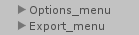
\includegraphics[scale=0.9]{./images/option_exp.png}
	
		La partie Client du réseau se divise en 2 parties, d'une part, l'adresse IP du serveur est renseignée, d'autre part le Client est créé.
		\subsubsection{Menu d'options}
		
\includegraphics[scale=0.9]{./images/option.png} Le composant principal du menu d'options est "IpInput", qui est composé d'un champ de saisie dans lequel une personne de l'IRISA doit renseigner l'adresse IP (IPv4) du serveur. Lorsque qu'une personne écrit dans le champ de saisie puis valide le texte en cliquant ailleurs ou en appuyant sur ENTREE, le script "getter" appliqué au GameObject de même nom enregistre la chaîne de caractères.
			Le "Placeholder" affiche un texte en grisé dans le champ pour guider la personne qui écrit.
		
		\subsubsection{Menu d'export}
		
\includegraphics[scale=0.9]{./images/export.png} Le menu d'export est utilisé une fois qu'une adresse ip a été renseignée dans le menu d'options.
			Le composant le plus important du menu d'export est le GameObject "exportScript" qui contient le script "Client".
			Le comportement de ce script est décrit ici:
			\begin{itemize}
				\item Si l'adresse IP renseignée n'est pas écrite dans un format IPv4 valide (XXX.XXX.XXX.XXX) alors le script lève une exception. Nous laissons le choix aux personnes de l'IRISA pour décider des actions dans l'exception.
				\item Un point de connexion IPEndPoint avec l'adresse IP renseignée et le port 80 sur lequel nous connectons un nouveau TcpClient pour établir la connexion, est créé.
				\item Un buffer d'octets qui contient les données du prefab ciblé par le "path" est créé.
				\item Les bytes contenus dans le buffer au serveur en utilisant un flux de données NetworkStream.
				\item Le flux de données est nettoyé.
			\end{itemize}

\section{Sauvegarder et Charger}
	\subsection{Sauvegarder}
		\subsubsection{Menu de sauvegarde}
		
\includegraphics[scale=1]{./images/save.png} Le menu de sauvegarde est déjà créé mais caché ainsi que la sauvegarde de la forme dans un prefab. Il reste à sauvegarder les textures dans le prefab. Il est conseillé de sauvegarder les prefabs dans un dossier "Resources" pour pouvoir utiliser la méthode "Resources.Load" pour charger un prefab.
	\subsection{Charger}
		\subsubsection{Menu d'ouverture}
			
\includegraphics[scale=1]{./images/load.png} Le menu d'ouverture est déjà créé mais caché, l'ouverture d'un prefab se fait dans le script "Load" appliqué au GameObject "Charger". Pour charger un GameObject  à partir d'un prefab il faut instancier le prefab comme s'il s'agissait d'un GameObject et renseigner le GameObject repère "parent" pour qu'il apparaisse.
\end{document}